Now far from being science fiction, robots are little by little entering our world. The tendency to replace humans with machines has existed for centuries, but it is only during the 20th century that technology has enabled us to achieve astonishing results.\\
Hence, the robots we know today come in different forms: from robots with human form, to mechanical arms, to robotic heads. 
In each case, there was extensive research and development before arriving at the results we can enjoy today.
Given the initial instability of robotic systems and the danger and cost, the creation of these devices went hand in hand with the development of special simulators. \\
It is indeed very inconvenient to repeat tests on hardware, for the reasons mentioned above. It is precisely in this circumstance that the need arises to simulate in a virtual environment the movements and actions that the robot would then have to repeat in the real world.
It is therefore necessary to set up a testing procedure that has precise specifications and is reliable and repeatable over time. \\
In particular, the simulated behaviour of the robot must be consistent with the measurements and physical specifications of the robot in order to have a reliable simulation.\\
From an automation engineering point of view, the main objective is to eliminate human intervention even on the testing procedure, in order to have a semi-autonomous testing software, which returns data that can be easily analysed both for internal development and for supply to third parties.\\
The operator must in any case monitor the progress of the test in order to obtain useful information on anomalous behaviour. 
This work proposes a tool for testing the navigation of a humanoid robot in a simulated environment, offering a faithful and secure solution and obviating the problematic testing on hardware.\\
In addition, lateral solutions are presented to problems that arose in the testing phase, such as the denoising of the image received from the robot`s video terminal.\\

\section{Oversonic Robotics}
This project has been realized as an application for Oversonic Robotics.\\
Oversonic Robotics is an Italian robotics start-up founded in 2020 in Besana in Brianza (MB) that wants to provide companies with intelligent systems that can assist humans in the most psychologically and physically demanding and exhausting jobs, thus enabling people to devote themselves to tasks that more effectively enhance intelligence.
Their first project, Robee (Figure \ref{fig:robee}), is an autonomous humanoid robot, 1.75 m tall with a weight of around 75 Kg. He operationally replicates the mechanical structure of the human body, with 36 movable joints and a complete set of sensors. This enables him to see and navigate the surrounding space. The interaction is managed via a voice interface, capable of carrying out a normal conversation. He has arms and hands that allow him to cover all kinds of tasks. These include the simplest gestures such as pointing or counting, to a solid grip for handling objects. For greater awareness of his surroundings and for better communication with operators, Robee is equipped with a variety of cameras that use facial recognition and object detection. 

\begin{figure}[H]
    \centering
    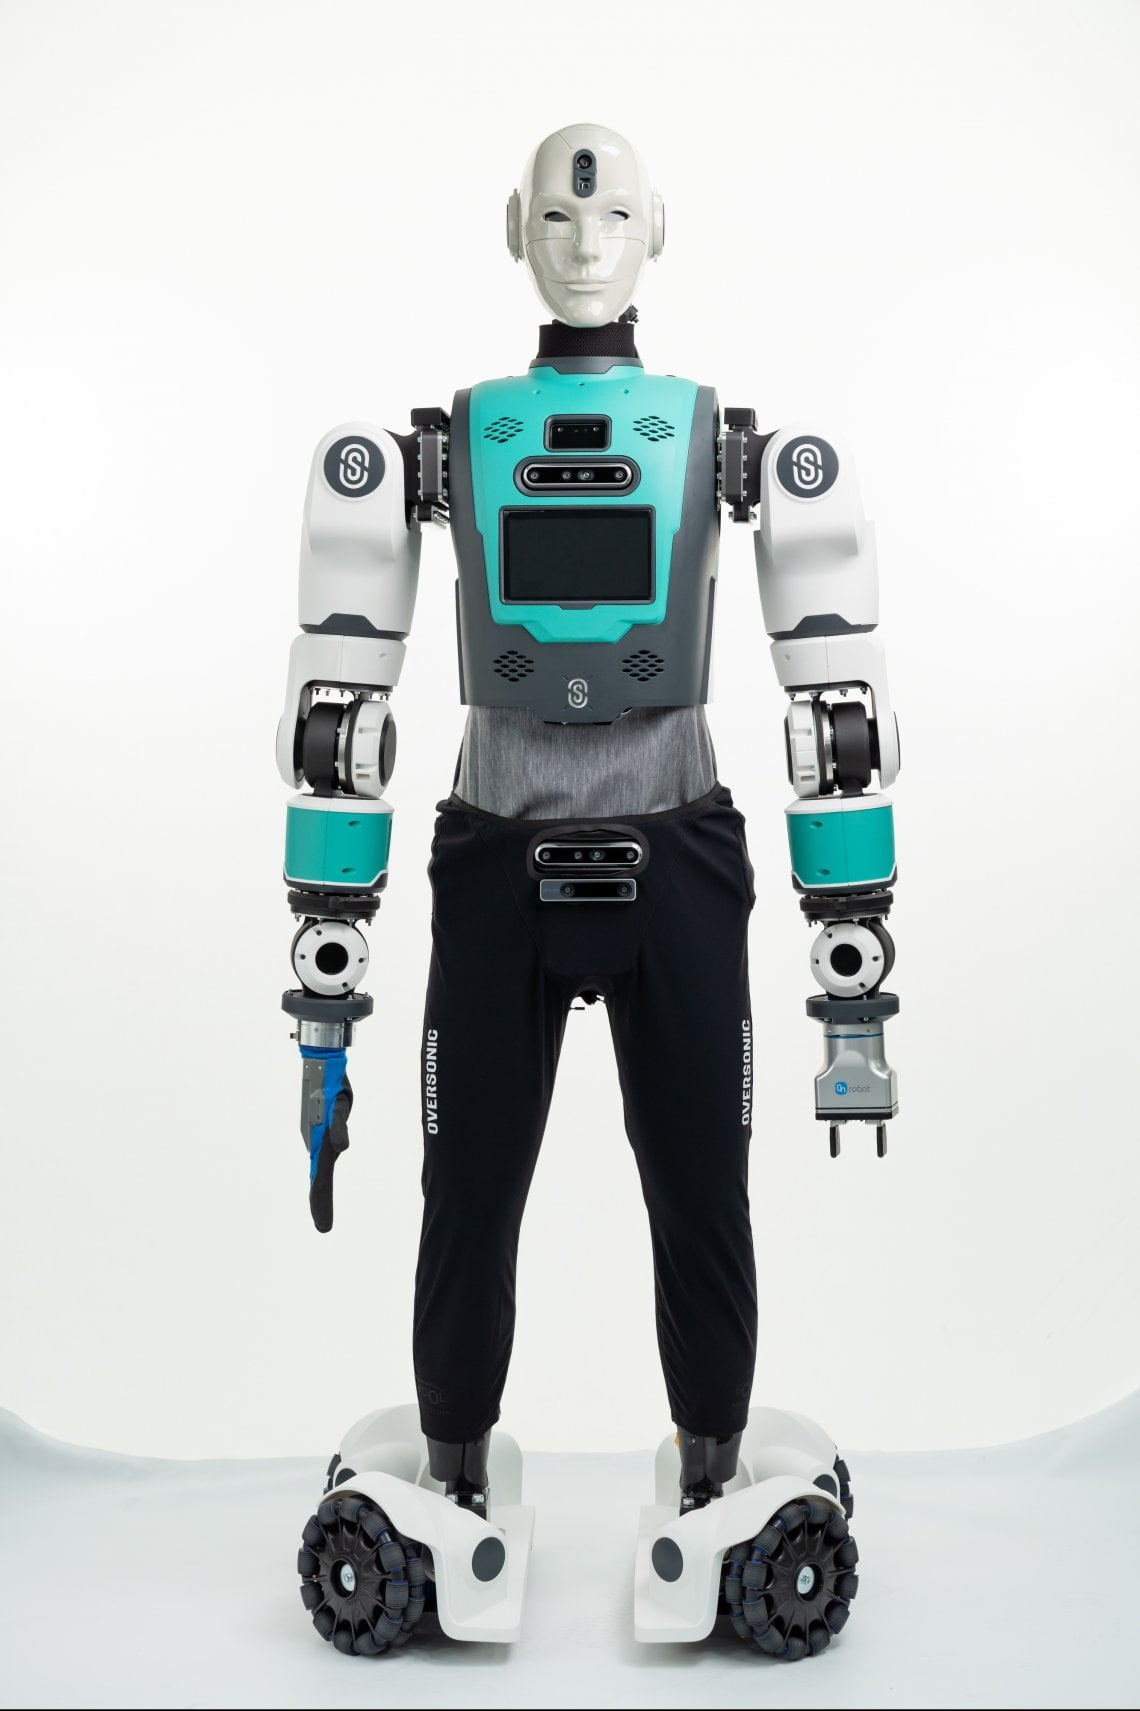
\includegraphics[scale=0.25]{Images/Chapter 1/robee_frontale.jpg}
    \caption{"Robee", the humanoid robot developed by Oversonic Robotics}
    \label{fig:robee}
    \citet{robeeimg}
\end{figure}
\section{Contribution}
The main contributions of this work are as follows:
\begin{itemize}
    \item Development of a simulated environment to test the robot's new navigation features. 
    \item Development of a module to test the navigation performance of the robot.
    \item Implementation of a point-cloud filter in order to improve obstacle handling and consequently navigation performance in critical brightness scenarios
\end{itemize}

\section{Document Structure}
The content is divided into two large sections: the first refers to the \textbf{Theoretical and Technological Background}, where the state of the art and the technologies used are introduced, in order to fully understand the system; the second one contains the \textbf{Contribution} of the thesis and
reports the architecture of the system, its implementation and results.
The thesis is composed of six chapters, below we list the content of each of them to give
the reader an overview of the work done.\\
\newline
\begin{itemize}
    \item Chapter \ref{ch:ros} provides an overview of the software platform ROS, Robot Operating
System, explaining its characteristic and philosophy that highlight why it is used as
common platform to manage robots’ operations, tasks, motions.
    \item Chapter \ref{ch:robot} first introduces robots providing a brief historical overview. It is then described Oversonic robot, Robee, describing its components, both software and hardware.
    \item Chapter 4 aims to introduce the literature survey of the various techniques used for
mobile robot navigation. Navigation and obstacle avoidance are one of the
fundamental problems in mobile robotics, here are described two type of control global
path planning and local motion control.
    \item Chapter 5 represents the main work of this thesis. It introduces first Gazebo simulator, afterwards it goes step by step through the building of the sim. robot and environment. It then encompasses the measurement module implemented. Results and issues are presented.
    \item Chapter 6 introduces point-cloud. This section proposes to solve an issue encountered while testing on the physical robot. 
\end{itemize}    






